\documentclass{article}
\usepackage[utf8]{inputenc}
\usepackage[czech]{babel}
\usepackage{graphicx}

\title{MoToX - uživatelská dokumentace}
\author{Kateřina Nevolová \\ \texttt{katka.nevolova@gmail.com} \\ 73502469}

\begin{document}
\maketitle

MoToX je jednoduchá 2D motokrosová plošinovka pro jednoho hráče, který ovládá malou motorku skrz méně či více složitý terén. Přitom musí navíc zneškodnit všechny nepřátelské objekty příručním plamenometem..

\section{Ovládání}

Program se spouští z terminálu příkazem \texttt{./motox}

Po spuštění programu se zobrazí menu s možností výběru konkrétního levelu. Samotná hra (motorka) se ovládá pomocí kurzorových šipek. Klávesou \texttt{up} ovládáme motorku směrem vpřed, \texttt{down} je brzda, \texttt{right} a \texttt{left} slouží k balancování a snažšímu pohybu motorkou po mapě. Mezerníkem pak stroj mění směr jízdy. Klávesou \texttt{x} se ovládá plamenomet. Hru lze kdykoliv opustit klávesou \texttt{esc}.

\section{Herní systém}

Po zvolení příslušného levelu hry z menu začíná hra. Na mapu se snesou nepřátelské objekty, které musí být zničeny pro úspěch dané mise.

Hráč může využít pro balancování ve složitch traťových situacích nejen všemožných salt a lopingů, ale také zavěšování samotné motorky za kolečko či (díky pokročilému vývoji výroby ochranných obleků) za hráčovu hlavičku.

Při průjezdu mapou čekají na hráče nebezpečné objekty, které musí bez dotyku zneškodnit. K tomu je samozřejmě motorka dobře vybavena.. mluvit zde bude napalm.

Hra končí vítězstvím, pokud hráč zneškodní všechny nepřátele, nebo naopak prohrou, pokud motorka spadne z mapy nebo se dostane moc blízko nepřátelům..

\section{Editace a tvorba map}
Do složky \texttt{maps} mohou být vkládány nové mapy. Soubor s mapou musí mít koncovku \texttt{.mtx}. Do samotného souboru je potom možné přidávat stěny a nepřátele:

\begin{itemize}
\item \texttt{w 1 1 3 1}
\begin{itemize}
\item Toto přidá stěnu (wall) ze souřadnice \texttt{1,1} do souřadnice \texttt{3,1}.
\end{itemize}
\item \texttt{e 2 1 0 -1 0.5 100}
\begin{itemize}
\item Toto přidá nepřítele (enemy) na souřadnice \texttt{2,1} o rychlosti \texttt{0} ve směru osy x a \texttt{-1} ve směru osy y (nepřítel bude tedy padat k zemi). Nepřátelský objekt bude mít velikost \texttt{0.5} a \texttt{100}hp (1 úspěšný zásah motorky ubírá 10hp).
\end{itemize}
\end{itemize}

Je třeba počítat s tím, že motorka se objeví okolo souřadnic \texttt{0,0} a je veliká zhruba jednu jednotku a tvorbu mapy tomu přizpůsobit.

\section{Screenshoty}
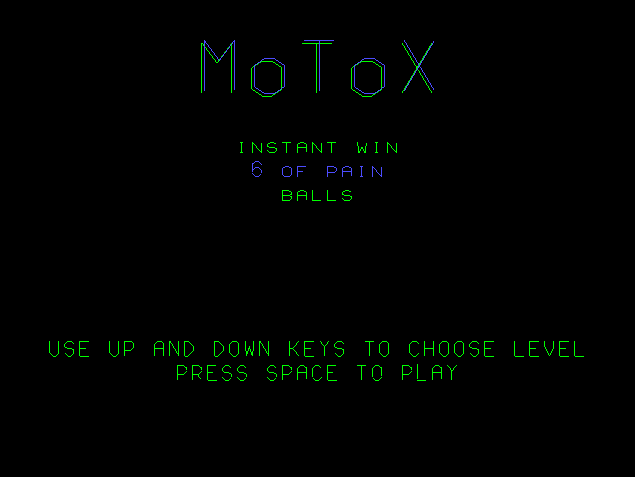
\includegraphics[width=6cm,height=4.5cm]{menu.png}
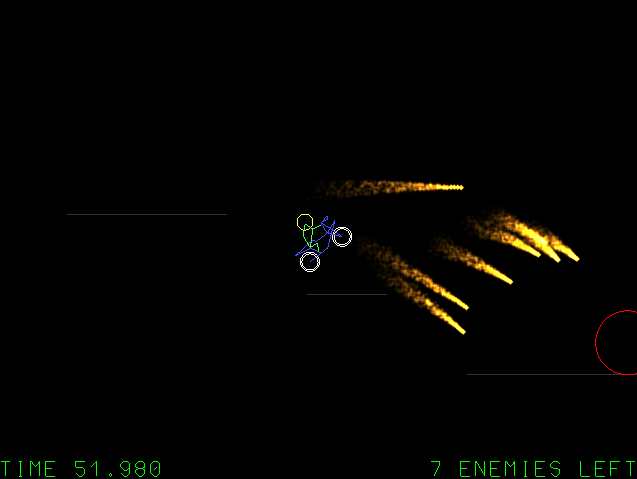
\includegraphics[width=6cm,height=4.5cm]{jump.png}
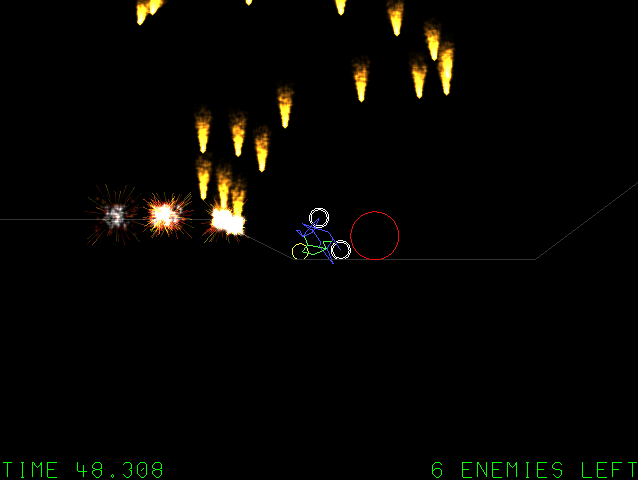
\includegraphics[width=6cm,height=4.5cm]{napalm_rain.png}
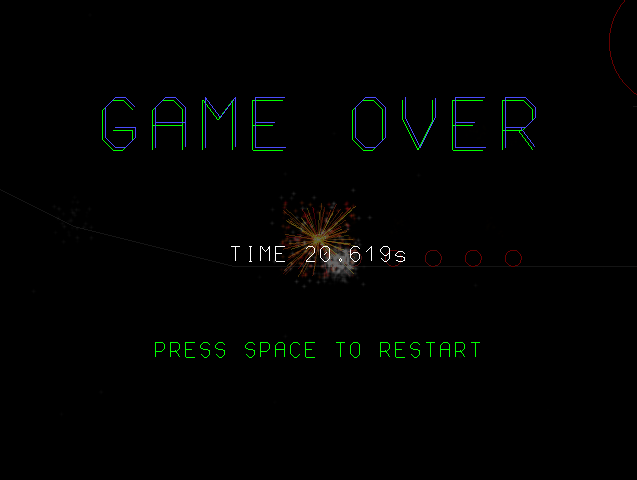
\includegraphics[width=6cm,height=4.5cm]{game_over.png}

\end{document}

